\chapter{Pilot reduction techniques for MIMO systems}
The current high gain frequency division duplex (FDD) Massive multiple-input, multiple-output (MIMO) systems pose several challenges to carry out the downlink beamforming. Specifically, downlink beamforming requires a channel estimation that usually needs long training and feedback overhead, scaling with the number of antennas at the base station (BS). 
%Also, FDD architectures, effective for symmetric traffic and delay-sensitive application, do not allow the use of uplink/downlink channel reciprocity to reduce downlink training, as in time division duplex (TDD) systems.
We exploit compressive sensing (CS) techniques to accurately estimate the channel, while assuring overhead reduction which is proportional to the sparsity level of the channel. The sparse virtual channel representation is obtained through the proposed dictionary design, which is more flexible, robust and able to estimate the cell characteristics. 
We specifically focus on massive MIMO-Orthogonal Frequency-Division Multiplexing (OFDM) systems that show more robustness to multipath fading, and analyze several CS algorithms to select among them the best technique with \textcolor{black}{the proposed dictionary design}.
Numerical results demonstrate that greedy solutions approach the basic pursuit bound with lower complexity and consequent shorter training period. The normalized hard thresholding pursuit (NHTP) technique is the greedy algorithm with the best performance complexity trade-off.	
Next-generation massive multiple-input multiple-output (MIMO) systems allow fine beamforming with narrow beams, thanks to the large number of antennas at the base station (BS) \cite{CommMag14} \cite{SPMag13}. This turns out in interference avoidance among users and higher throughput compared to current architectures. 

However, to achieve effective downlink beamforming, precise channel state information (CSI) is required. In time-division duplexing (TDD) systems, CSI can be estimated exploiting channel reciprocity \cite{LearningCS15}. Specifically, the uplink channel information, obtained easily due to the low number of antennas at the mobile station, can be exploited for downlink beamforming. 

On the contrary, frequency-division duplexing (FDD) architectures do not allow the use of channel reciprocity since different frequency bands are used for uplink and downlink with consequent different channels. Since FDD systems are more suitable for delay-sensitive and symmetric traffic systems, new solutions for dowlink training overhead reduction are needed.  
On this purpose, the compressive sensing (CS) framework can be exploited to reduce the downlink training period, by sparsely representing the channel response with some dictionary or basis.

The discrete Fourier transform (DFT) matrix has been already employed to
represent the channel in a sparse manner \cite{SpatSparse} \cite{SPTrans14}. However, such representation is not valid for all the antenna geometries, but only for uniform linear array (ULA) with a sufficient number of antennas and limited scattering, which reduces its real feasibility.

\textcolor{black}{New dictionary based virtual channel model have been proposed to sparsely represent the channel}, which are able to adjust to the cell characteristics, with no restriction to the array geometry. We exploit dictionary for sparse channel model and, once sparse channel representation is obtained, we apply compressive sensing techniques for channel estimation with a reduced dowlink training period.

We specifically focus on MIMO-orthogonal frequency division multiplexing (OFDM) systems. In order to mitigate the frequency selective fading, OFDM is used along with MIMO effectively converting it into flat fading channel. Each subcarrier is transmitted over a narrow band hence simplifying equalizer design at the receiver. 
We compare different compressive sensing techniques, i. e., convex optimization based approaches (basic pursuit (BP)) and greedy methods (matching pursuit (MP)). Among the greedy algorithms, we employ the well known orthogonal matching pursuit (OMP), as well as the iterative hard thresholding (IHT) and the normalized hard thresholding pursuit (NHTP) methods.

The main contributions of this work are:

\begin{enumerate}
	\item a compressive sensing based solution is proposed for channel estimation in massive MIMO-OFDM FDD systems with reduced downlink training overhead;
	\item we implement different CS algorithms and choose the optimal one with \textcolor{black}{ the proposed} dictionary, while \cite{LearningCS15} only demonstrates the usefulness and potential of dictionary learning based channel modeling applied to an OMP CS solution, without analyzing the problem of optimal CS algorithm selection for massive-MIMO using learned dictionary;
	\item a comparison of DFT basis and \textcolor{black}{proposed} dictionary is presented varying the pilot spacing, which shows that \textcolor{black}{proposed} dictionary based compressed sensing is more robust and reliable even when increasing pilot spacing. 
	\item  simulation results show that the basic pursuit gives the best performance at the cost of high complexity. Greedy solutions approach the basic pursuit bound with a lower complexity and consequent shorter training period. Specifically, the NHTP approach is the greedy algorithm with the best performance complexity trade-off.
\end{enumerate}
\section{System Model}
\label{SM}
 Wireless channel involves multiple paths of varing delays and gains. The transmission at high data rates generally implies a small symbol duration, so that the received signal  is affected by intersymbol interference (ISI) of successive modulation symbols, due to several paths in the propagation environment. A time varying channel with $L_t$ paths can therefore be represented as 
 \begin{equation}
h(t)=\sum_{k=0}^{L_t-1}\alpha_k\delta(t-\tau_k)
 \end{equation}
 Where $\tau_k$ and $\alpha_k$ denote the $k^{th}$ channel path delay and complex gain respectively. In order to combat multipath fading, the well known multicarrier scheme OFDM may be used, by employing narrow spaced subcarriers at the transmit side. An OFDM signal consists of $N_o$ subcarriers, equally frequency spaced at ${\Delta} f=\dfrac{1}{T_s}$, with $T_s$ the sampling time.
  An OFDM discrete time baseband signal can be expressed as 
  \begin{equation}
S_i(n)=\dfrac{1}{\sqrt{N_o}}\sum_{k=0}^{N_o-1}x_i(k)e^{j\dfrac{2\pi kn}{N_o}}
  \end{equation}
  where $S_i(n)$ represents the $n^{th}$ sample of the $i^{th}$ OFDM symbol, and $x_i(k)$ represents the data transmitted over the $k^{th}$ subcarrier in the $i^{th}$ symbol interval, while $\dfrac{1}{\sqrt{N_o}}$ is a normalization factor.
The $k^{th}$ subcarrier in the equivalent lowpass domain is described by the signal $g_k(t)$ as
\begin{equation}
g_k(t)= e^{j2\pi{\Delta}fkt}\cdot rect(\dfrac{t}{T_s})
\end{equation}
Despite the fact that these subcarriers overlap each other, they do not interfere since they are orthogonal. 
The maximum channel delay $\tau_{max}=\tau_{L_t-1}$ may cause intercarrier interference (ICI) which is usually mitigated by appending a cyclic extension of each OFDM symbol at its end, for a number of samples $G_i\ge \tau_{max}$, i.e. the guard interval.
Therefore, the OFDM total symbol duration is $T_{sym}=(N_o+G_i)\cdot T_s$
A perfect channel knowledge is a fundamental requirement for channel equalization. 
%\textcolor{red}{PLEASE, ADD SPACES AFTER PUNCTUATION AND/OR WHERE NEEDED}
The channel may be usually estimated by blind or pilot based techniques. In OFDM pilot based channel estimation, pilots are arranged in a time frequency grid over time (block based) or frequency (combo based). The receiver can directly estimate channel behavior at the frequencies where pilots are transmitted using conventional least square based technique
%\textcolor{red}{THIS EQUATION SHOULD BE CHANGED ACCORDING TO (4)} 
\begin{equation}
H_{i,k}=\dfrac{R_{i,k}}{S_{i,k}}
\end{equation}
Where $S_{i,k}$ is $k^{th}$ position of $i^{th}$ OFDM symbol transmitted and  $R_{i,k}$ is $k^{th}$ position of $i^{th}$ OFDM symbol received.
 Recently, research has been focused on exploiting communication channel sparsity, considering the fact that channel exhibit only few dominant propagation paths which may be approximated as a linear combination over a known basis or dictionary, resulting in a sparse Channel impulse response (CIR). Traditionally DFT basis are used for sparse channel representation. 
	\[
 \mathbf{	\phi=
	\begin{bmatrix}
e^{-j2\pi k_{0,1}} &\dots& e^{-j2\pi k_{0,N_o-1}} \\
e^{-j2\pi k_{1,1}} &\dots& e^{-j2\pi k_{1,N_o-1}} \\
\vdots & \ddots & \\                                                                                     
%e^{-j2\pi k_{L-1,1}/\tau_1} &\dots& e^{-j2\pi k_{L-1,M}/\tau_M} \\
e^{-j2\pi k_{N_o-1,1}}  &\dots& e^{-j2\pi k_{N_o-1,N_o-1}} \\
	\end{bmatrix}}
	\]	
The use of the DFT base is compliant with the theoretical results of signals estimation in CS\cite{Candes08}, and it has been used to represent sparse channel models. However, DFT basis may represent the channel only in a few, although orthogonal, directions. In order to better estimate the channel, more robust and refined basis may be defined.\\
\subsection{Sparse Channel Estimation}
\label{SparseChannelEstimation}
In this work, we will focus on a downlink massive MIMO-OFDM system, with a number of transmit antennas equal to $N$, and a single antenna at the receiver. \textcolor{black}{Multicarrier OFDM modulation is used in order to mitigate frequency selective fading and aid channel estimation by means of pilot subcarriers. Data frames are represented by $\mathbf{d}_j$ with $j = 1,...,N-L$, while the number of training pilots is $L$.}
\textcolor{black}{
\begin{equation}
\mathbf{x}=\{\mathbf{P}_1 ,\mathbf{d}_1 ,\mathbf{P}_2 ,\mathbf{d}_2,...,\mathbf{P}_L,...,\mathbf{d}_{N-L}\}
\end{equation}
}
\textcolor{black}{
Pilots P are built according to a Rademacher distribution (RD), comprising equally likely symbols belonging to [+1,-1] and multiplied by a phase rotation as in the following equation.
\begin{equation}
\mathbf{P} = [\mathbf{p}_1e^{-j\pi l_1},\mathbf{p}_2e^{-j\pi l_2},...,\mathbf{p}_Le^{-j\pi l_L}]
\end{equation}
where $l_j$ are uniformly distributed random numbers belonging to the interval $[0,1]$
}, while the channel delay profile can be formulated using OFDM sample time and guard interval for each dictionary point as follows
	\begin{equation}
\bm{\tau}_h=[0,\alpha,2\alpha,\cdots \cdots (M-1)\alpha]
	\end{equation}  

where $M$ is the dictionary length and $\alpha=G_i\cdot T_s-G_i\cdot T_s/M$ is the minimum channel spacing which is calculated by considering the constraint that $\tau_{max}$ must not exceed $G_i$. 
The downlink channel vector $\mathbf{h}\in \mathbb{C}^{N\times 1}$ is estimated at the mobile receiver by using pilot symbols, and this channel  state information is sent back to the base station \cite{LearningCS15}.

In more details, the transmitted pilot symbols may be represented by the matrix $\mathbf{A} \in \mathbb{C}^{LxN_o}$, for DFT based sensing matrix and $\mathbf{A} \in \mathbb{C}^{LxM}$ for dictionary based sensing matrix. Block based pilot arrangement is used as it is most suitable for multipath fading channel. For example, for $N_o$ equals to 2048, 32 pilots are transmitted per OFDM symbol with pilot interval (PI) equal to 64, while the remaining 2016 sub carriers are used for data. After the OFDM DFT matrix multiplication, the received signal at each single user can be expressed as in the following:
\begin{equation}
\mathbf{y}=\mathbf{Ah}+\mathbf{n}
\end{equation}
where the elements of $\mathbf{n}\in \mathbb{C}^{Lx1}$ are additive white Gaussian Noise (AWGN) samples with variance $\sigma^2_n=N_0/2$.
Least square (LS) channel estimation requires a number of pilot symbols $L\ge N$, needed to compute the pseudoinverse of the pilot matrix $\mathbf{A}$. For massive MIMO the large number of Antennas $N$ can make this unfeasible, considering also that the estimated channel information shall be sent back to the base station. 
\subsection{Sparse Channel Representation}
\label{SparseChannelRepresentation}
\textcolor{black}{If $L<N$ the compressed sensing paradigm may be taken under consideration, since channel estimation may be viewed as measuring a high dimensional signal with a very limited number of measurements, assuming that the original signal, i.e. the channel estimate $\mathbf{h}$, may be sparse in a some suitable basis.\\
In order to construct the dictionary $\mathbf{D}$ basis, we are only considering the useful OFDM symbol duration, without $G_i$, and taking the channel delay profile into account\\
\textcolor{black}
{
	\[
\mathbf{	D=
	\begin{bmatrix}
	e^{-j2\pi \cdot1 \tau_1} & e^{-j2\pi\cdot1 \tau_2}&\cdots& e^{-j2\pi \cdot1 \tau_M} \\
	e^{-j2\pi \cdot2 \tau_1} & e^{-j2\pi\cdot2 \tau_2}&\cdots& e^{-j2\pi \cdot2 \tau_M} \\
	\vdots & \dots & \\                                                                                     
	%e^{-j2\pi k_{N_o-1,1}\tau_1} & e^{-j2\pi k_{N-1,2}\tau_2} &\cdots& e^{-j2\pi k_{N-1,M}\tau_M} \\
	e^{-j2\pi\cdot N_o\tau_1} & e^{-j2\pi \cdot N_o\tau_2} &\cdots& e^{-j2\pi \cdot N_o\tau_M} \\
	\end{bmatrix}}
	\]
where 
$\tau(m)=  1/T_{sym}\cdot \tau_h(m)$  where $m=\{0,1,\cdots,M-1\}$
}
Following this reasoning, to effectively represent channel sparsity, if the basis $\mathbf{D}\in \mathbb{C}^{M\times N_o}$ may be redefined such that $\mathcal{D}=\mathbf{D}_{LxM}$ is a sub-matrix of $\mathbf{D}$, we can then write\\
%  where the representation vector $\mathbf{\beta}\in \mathbb{C}^{L\times 1}$ is a compressed vector, the downlink channel estimation can be written as \cite{LearningCS15}:
%$\mathbcal{D}$\\ 
\begin{equation}
\label{sparseChannel}
%\mathbf{y}=\mathbf{Ah}+\mathbf{n}
\mathbf{y}=\mathbf{Ah}+\mathbf{n}=\mathcal{D}\cdot P\beta+\mathbf{n}
\end{equation}
\textcolor{black}{
 where $\mathbf{\beta}\in \mathbb{C}^{L\times 1}$ is a representation compressed vector, and $\mathbf{y} \in \mathbb{C}^{M\times 1}$ the estimated one. 
 The design of dictionary $\mathbf{D}$ and sensing matrix $\mathbf{A}$ is always critical when using compressed sensing. It can be seen that $\mathbf{D} \in \mathbb{C}^{N_oxM}$, and $\mathbf{A} \in \mathbb{C}^{LxM}$ is basically consisting of some specific rows of $\mathbf{D}$ related to pilot locations as in \cite{review17}:
	\begin{align}
	\mathbf{A} &= 
	\begin{matrix}
	\begin{bmatrix}
	e^{-j2\pi l_1 \tau_1} &\cdots& e^{-j2\pi\cdot l_1\tau_M} \\
	e^{-j2\pi l_2\tau_1} &\cdots& e^{-j2\pi\cdot l_2\tau_M} \\
	\vdots & \ddots & \\                                                                                     
	%e^{-j2\pi L-1/\tau_1} &\dots& e^{-j2\pi k_{L-1,M}\tau_M} \\
	e^{-j2\pi l_L \tau_1}  &\cdots& e^{-j2\pi \cdot l_L\tau_M} \\
	\end{bmatrix}
	\begin{bmatrix}
	 p_1e^{-j\pi l_1}\\
	 p_2e^{-j\pi l_2}\\
	 \vdots\\
	 p_Le^{-j\pi l_L}
	\end{bmatrix}
	\end{matrix}
	\end{align}
	For comparison purposes, the sensing matrix $\mathbf{A}$ with dft basis $\mathbf{\phi}$ is computed in a similar manner from $\mathbf{D}$, i.e. only some specific rows of the basis function related to the training subcarriers are considered:}
  \textcolor{black}{
 	\begin{align}
 	A_\phi &= 
 	\begin{matrix}
 	\begin{bmatrix}
 	e^{-j2\pi k_{l_1,1}} &\dots& e^{-j2\pi k_{l_1,N_o}} \\
 	e^{-j2\pi k_{l_2,1}} &\dots& e^{-j2\pi k_{l_2,N_o}} \\
 	\vdots & \ddots & \\                                                                                     
 	%e^{-j2\pi k_{L-1,1}/\tau_1} &\dots& e^{-j2\pi k_{L-1,M}/\tau_M} \\
 	e^{-j2\pi k_{l_L,1}}  &\dots& e^{-j2\pi k_{l_L,N_o}} \\
 	\end{bmatrix}
 	\begin{bmatrix}
 	p_1e^{-j\pi l_1}\\
 	p_2e^{-j\pi l_2}\\
 	\vdots\\
 	p_Le^{-j\pi l_L}
 	\end{bmatrix}
 	\end{matrix}
 	\end{align}}}
 \textcolor{black}{
The equivalent channel representation in (\ref{sparseChannel}) is sparse if $||\mathbf{\beta}||_0=s\ll N$. Further, if we are able to solve for compressed vector $\mathbf{\beta}$, then the channel estimate can be obtained.
 %as $\hat{\mathbf{h}}=\mathbf{A\beta}$ to build channel at all locations learned from $\mathbf{\beta}$.
 Additionally, sparse signal reconstruction is based on the assumption that $\mathbf{h}$ is a s-sparse CIR, i.e. its channel energy is uniformly distributed among few dominant taps. The exact position of these dominant taps is not a priori known, and it must be estimated for effective channel sensing \cite{review17}.\\
Sensing matrix $\mathbf{A}$ can be represented in the form of a DFT basis $\mathbf{\phi}\in \mathbf{C}^{N_o\times N_o}$ or in  the form of an overcomplete dictionary  $\mathbf{D}\in \mathbf{C}^{N_o\times M}$, to solve a channel estimation problem with $M>N_o$.\\
The main objective of any dictionary is to sparsely represent data in terms of some basic elements, called atoms, that are not required to be orthogonal and they may be seen as an over-complete spanning set.
The basic philosophy of these algorithms is that a dictionary may be inferred from input data, inspired by the fact that we need to represent each data set by using as few samples as possible. \\
To solve the sparse channel estimation problem, each iteration alternatively minimizes the CS error.
%with respect to  either $\mathbf{D}$ or $\mathbf{\beta}$, while keeping the other fixed\cite{LearningCS15}.
The algorithm convergence depends on the specific sparse recovery and dictionary in the algorithms. Our work aims to obtain optimal estimate starting from an overcomplete dictionary representation.
Finally, a channel estimate is built at all location merely from dictionary $\mathbf{\hat{x}=Dy}$. }
\section{COMPRESSIVE SENSING METHODS}
\label{formulation}
We apply different CS algorithms to the \textcolor{black}{proposed dictionary based} sparse channel representation, in order to select the best CS solution able to reconstruct the estimated channel from few measurements.
CS methods can be categorized broadly into convex relaxation iterative algorithms \cite{Donoho06}, \cite{Candes08}, and greedy ones \cite{Masood13}, \cite{Dai09}. Other methods have been proposed as a combination of these techniques \cite{Donoho12}, \cite{CoSaMP09}, \cite{Wang12}. 
\subsection{Convex relaxation iterative algorithms} 
The convex relaxation type exploits linear programming to solve undetermined systems.
Some CS techniques are formulated as $\mathcal{L}_0$, $\mathcal{L}_1$, and $\mathcal{L}_2$ norm minimizations. 
In the following, we denote with $\mathbf{x}$ the estimated channel response $\hat{\mathbf{h}}$.
Considering the basic pursuit algorithm, the solution of a $\mathcal{L}_1$ norm minimization can be formulated as a cost function minimization problem. 
BP is an iterative algorithm that initializes the first guest ($\mathbf{x}=\mathbf{x}_0=\mathbf{A}^T\mathbf{y}$), which represents the minimal signal energy, and then computes the cost function by minimizing $\|\mathbf{y}-\mathbf{A} \mathbf{x}_0\|_2$. 
For the next $i$ iterations, the measurement matrix is calculated selecting the $s$ required measurements, and the signal coefficients are adjusted according to the minimized form. The iterations stop when enough signal coefficients are obtained, less than its sparsity level \cite{Phy16}. 

Convex relaxation methods needs only a small number of measurements to reconstruct the signal; anyway, they exhibit a greater complexity in terms of computation and time consuming \cite{Phy16}.

\subsection{Greedy algorithms} 

Differently from the convex optimization algorithms, greedy techniques are easy to implement and able to quickly recover a sparse signal, although their solution is not optimal \cite{Phy16}. Such methods are in line with our objective to reduce the downlink training overhead for channel estimation, however we should also strictly take into account their performance.

Let us call $\mathbf{x}$ the large dimensional signal, that is the channel to be estimated in our case, with a high number $M$ of samples, which is sparse in some domain. 
Greedy algorithms pick one position of a non-zero element of $\mathbf{x}$, which corresponds to select one column from the measurement matrix. 

Some techniques have been proposed under this category: orthogonal matching pursuit (OMP) \cite{Sensing14}, compressive sampling matching pursuit (CoSaMP) \cite{CoSaMP09}, iterative hard thresholding (IHT) \cite{IHT09}, and normalized hard thresholding pursuit(NHTP) \cite{Greedy08}. 
Matching pursuit selects a column from the measurement matrix that maximizes the inner product of the current residuals. As a first step, the algorithm selects from the dictionary the vector corresponding to the longest projection of $\mathbf{x}$. In the second step, the signal $\mathbf{x}$ is orthogonalized by removing any element of the selected vector from $\mathbf{x}$ in order to obtain its residual with the lowest energy. 
Finally, such two steps are iteratively processed
for the remaining part of the dictionary until the residual norm is lower than a certain threshold \cite{Phy16}.
Orthogonal matching pursuit method is a variant of the
matching pursuit algorithm by discharging both the elements of the selected vector from $x$, and from the
basis, before doing again the process. 
Orthogonal matching pursuit shows better results than
matching pursuit, at the cost of a higher computational complexity.

Given the high-dimensional signal $\mathbf{x}$, observed via low-dimensional measurements $\mathbf{y}$, the aim is to reconstruct the signal from the measurements.
Iterative Hard Thresholding (IHT) is a simple algorithm based on thresholding\cite{HTP11}:
\begin{itemize}
	\item solving the rectangular system $\mathbf{A}\mathbf{x} = \mathbf{y}$ is equivalent to solve the square system $\mathbf{A}\cdot \mathbf{A}\mathbf{x} =\mathbf{A}\cdot \mathbf{y}$;
	\item a sequence $\mathbf{x}^i$ can be defined as a recursion $\mathbf{x}^{i+1}=(\mathbf{I}-\mathbf{A}\cdot \mathbf{A})\mathbf{x}^i$;
	\item given the objective of sparse vectors, each step includes the hard thresholding operator that keeps $s$ nonzero largest components of a vector and fixes the other ones to zero.
\end{itemize} 

Compressive Sampling Matching Pursuit algorithm pursues first a suitable candidate for the support, and then finds the vector, with this support, that fits well the measurements \cite{HTP11}. 

The Hard Threshold Pursuit (HTP) algorithm is a combination of the IHT and the CoSaMP or Subspace Pursuit algorithms \cite{HTP11}, so that it selects the $s$ largest component of $\mathbf{x}^{i}+\mathbf{A}\cdot\mathbf{A}(\mathbf{x}-\mathbf{x}^i)\approx\mathbf{x}$.
The HTP main feature is its high speed.

Finally, Normalized Hard Thresholding Pursuit is a variant of the HTP method.

\section{PERFORMANCE EVALUATION}
\label{Perf}
In this section, the performance of the proposed scheme are evaluated for different CS techniques.

\subsection{Simulation Setup}
\label{SimSetup}
We consider a MIMO-OFDM system, with $100$ transmit antennas and one receive one. The base station uses $256$ OFDM subcarriers for downlink transmission. Some subcarriers are employed for pilot sequences and others for data. The multipath channel length $L_{taps}$ is equal to $6$, whose consequent interference is directly solved by the OFDM guard interval, whose  length is set equal to $16$. Table \ref{tabSim} summarizes the system parameters.
\begin{table} \footnotesize
	\renewcommand{\arraystretch}{1.1}
	\caption{Simulation parameters}
	\label{tabSim}
	\centering
	\begin{tabular}{llr}
		\textbf{Parameter}&\textbf{Symbol}&\textbf{Value}\\
		\hline
		\\
		Transmit antennas & $N$&$100$\\
		Receive antennas & $R$&$1$\\
		OFDM subcarriers & $N_o$&$256$\\
		OFDM guard interval & $G_i$&$16$\\
		QAM Modulations & $QAM$&$32$\\
		Multipath channel length & $L_t$&$6$\\
	\end{tabular}
\end{table}
\subsection{Performance Analysis}
\label{PerfAnalysis}
\textcolor{black}{
Wireless channel in the angular domain can be represented by sparse DFT basis as reported in \cite{review17},\cite{pilot15}. Although DFT basis are orthonormal, only a few angles or directions may be defined in it. In practical systems, signals may arrive from any arbitrary directions, so predefined patterns of dft bins do not represent a good choice \cite{LearningCS15}. On the contrary, in the proposed solution, a dictionary with more refined bins is used in order to estimate the sparse channel model. In Fig. 1 and 2, the angular representation of DFT and Dictionary basis are shown, for a $N_o \times N_o$ DFT matrix and a $N_o \times M$ dictionary one. If $N_o = M$ the dictionary is defined as complete, while when $M>N_o$ the dictionary is said over-complete, providing more redundant basis which is more flexible to estimate the channel.}
\begin{figure}
	\centering
%	\includegraphics[width=1\linewidth]{dict_angles.eps}
	\includegraphics[width=60mm,height=60mm]{figures/figchap4/dict_angles.eps}
	\caption{Analysis of angles of dictionary basis 16x20}	
	\label{Fig_result1}
\end{figure}
\begin{figure}
	\centering
%	\includegraphics[trim=1cm 6.1cm 6cm 14.0cm, clip=true, scale=0.6]{dft_angles.eps}
	\includegraphics[width=60mm,height=60mm]{figures/figchap4/dft_angles.eps}
	\caption{Analysis of angles of dft basis 16x16}	
	\label{Fig_result1}
\end{figure}

The effects of Different pilot spacing and sparsity levels on on system performance are analyzed. In massive MIMO, pilot training overhead is one of the main concern, since it is proportional to the number of transmit antennas, in order to acquire good CSI at the base station. 

In Fig. \ref{Fig_result1}, we analyze the effects of the OMP algorithm on BER for the following different values of the sparsity level $s= 15$, $30$, $45$, $60$, $65$. We also observe the system performance for pilot interval (PI) values equal to $4$, $14$. Similar analysis can be also conducted for the other CS techniques.
Fig. \ref{Fig_result1} shows that \textcolor{black}{the proposed dictionary} performs better than the DFT based one, and it is more robust to pilot spacing changes. Indeed, when $PI=14$, the DFT basis performance behaves worse than $PI=4$, while the dictionary based algorithm almost maintains the same performance. 
Further, when the sparsity level $s$ is increasing, all the channel measurements are more accurately represented, indeed the bit error rate is decreasing.

\begin{figure}
	\centering
	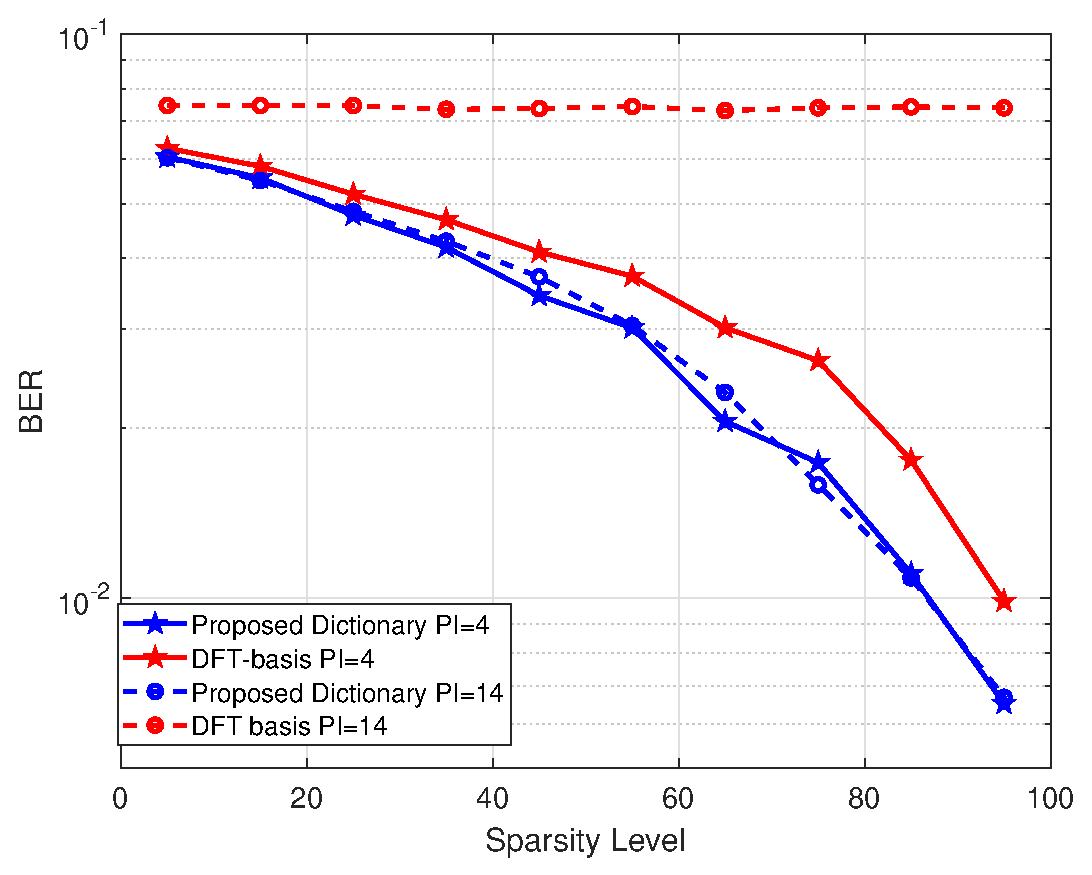
\includegraphics[width=110mm,height=80mm]{figures/figchap4/sparsity.eps}
	\caption{Analysis of DFT basis and \textcolor{black}{proposed} dictionary with different sparsity levels $s$ and pilot spacing for OMP algorithm}	
	\label{Fig_result1}
\end{figure}


Although there is a huge list of compressed sensing algorithms, having different benefits and drawbacks that are suitable for different systems/models, and with distinct convergence and complexity constraints, in the following figures we focus on some prominent greedy CS techniques, i. e., OMP, CoSaMP, IHT, NHTP \textcolor{black}{with dictionary,} compared to convex optimization based basic pursuit algorithms.

%\textcolor{blue}{Some greedy algorithms choose the elements that best approximate the signal at each iteration in a greedy fashion. While greedy thresholding algorithms choose such elements by fixing a threshold at each iteration and evaluating the elements that exceed such threshold in magnitude.}
%\textcolor{red}{We compare several compressed sensing algorithms with learned dictionary and DFT basis in order to find the best solution in terms of performance (BER) and complexity. CUT???} 

Fig. \ref{Fig_result2} illustrates the performance of CS algorithms with \textcolor{black}{the proposed dictionary}, showing that the basic pursuit method outperforms all the considered greedy algorithms in terms of BER, while the least square estimation (LSE) approach gives the worst performance. However, the curve of the greedy NHTP is really close the BP one, with the advantage of high computational complexity reduction.
Indeed, there is a trade-off between performance and computational complexity that we need to take into account, as shown in Sec. \ref{ComplexAnalysis}.
%\begin{figure}[ht]
%	\centering
%	\includegraphics[width=1\linewidth]{PI-4It-20Tx-100mod-32GI-16_iht.eps}
%	\caption{BER vs SNR for transmit antennas $N=100$, receive antenna $R=1$, number of channel taps $L_{taps}=6$}	
%	\label{Fig_result2}
%\end{figure}

\begin{figure}
	\centering
	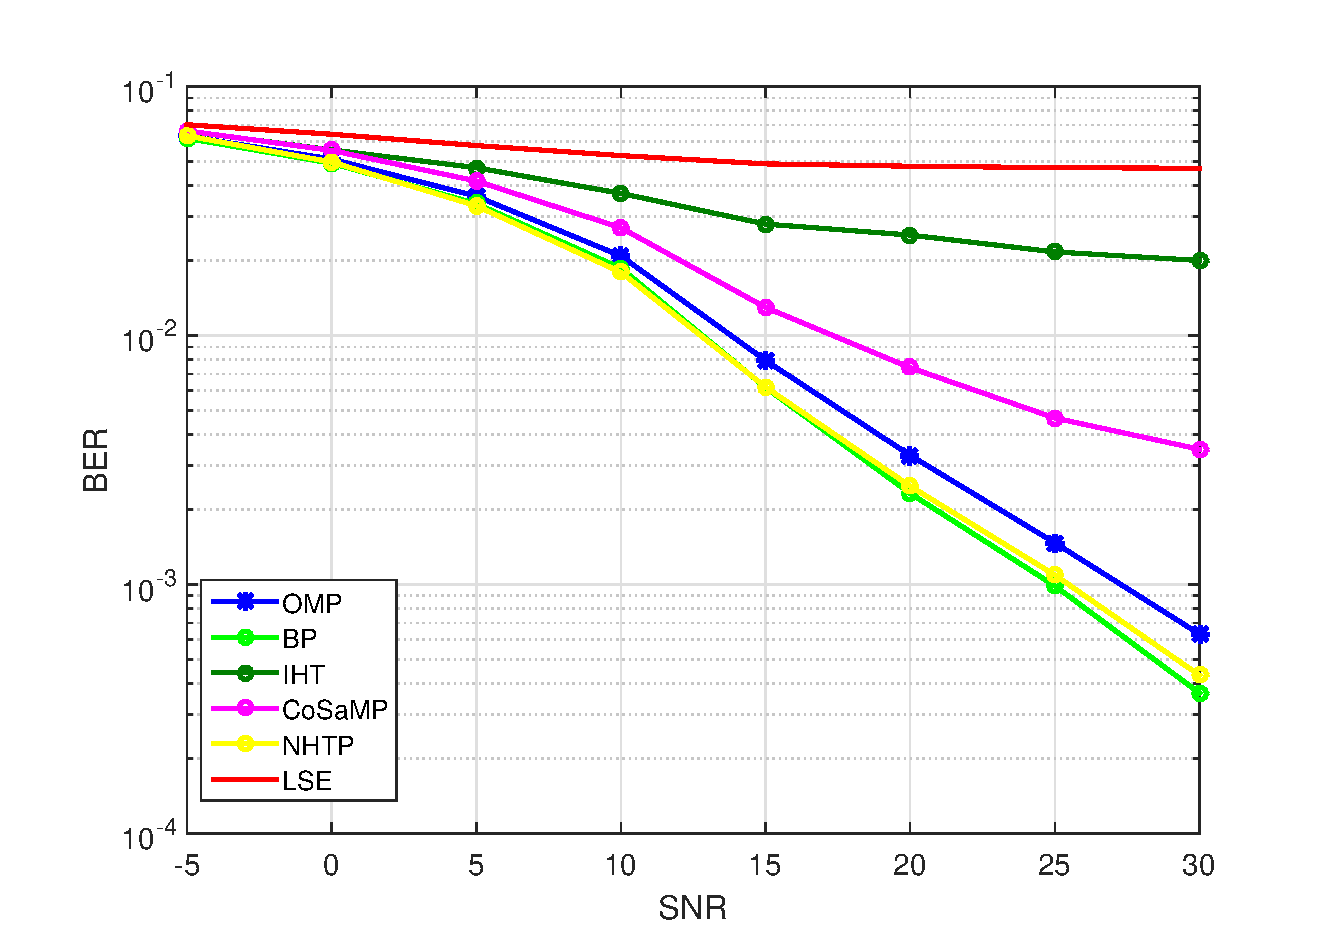
\includegraphics[width=120mm,height=85mm]{figures/figchap4/Fig2b.eps}
	\caption{Performance of CS techniques with \textcolor{black}{dictionary basis}: BER vs SNR (dB) for transmit antennas $N=100$, receive antenna $R=1$, number of channel taps $L_t=6$}	
	\label{Fig_result2}
\end{figure}

Finally, in Fig. \ref{Fig_result3} we analyze the effect of multipath channel for the NHTP \textcolor{black}{with the proposed dictionary} by varying the number of channel taps. We focus only on this algorithm since it is the best choice in terms of performance complexity trade off, as detailed in the following.

\begin{figure}
	\centering
	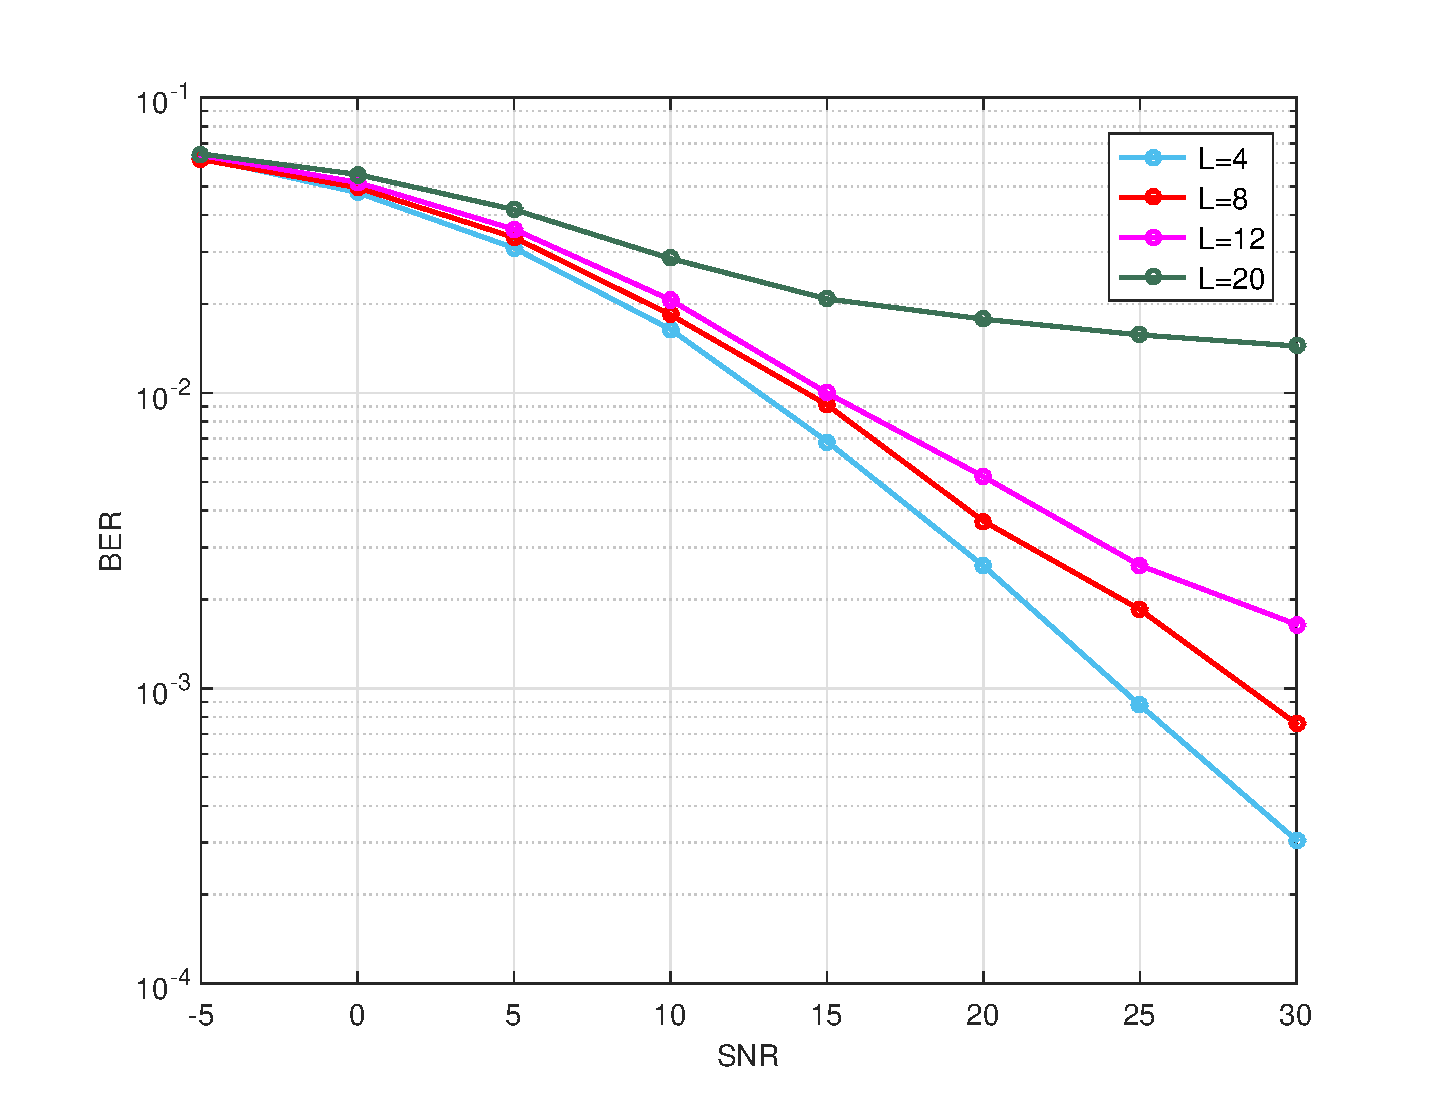
\includegraphics[width=120mm,height=85mm]{figures/figchap4/htp_L_1.eps}
	\caption{BER vs SNR (dB) for NHTP algorithm \textcolor{black}{with dictionary} changing the number of channel taps}	
	\label{Fig_result3}
\end{figure}
\textcolor{black}{
		Pilot overhead reduction has been compared among different compressed sensing based algorithms including convex optimization based BP and other greedy algorithms. It has been observed that the performance curve rapidly move down with decreasing pilot interval. The previous work \cite{pilot15} investigated pilot overhead reduction using CS based algorithm by random pilot allocation at different subcarriers for each antenna. They have used random sending matrix with DFT basis for sparse channel representation. In this section, we have assumed the same parameter setting for comparison purposes: transmit antennas = 128, number of subcarriers = 2048, SNR equal to 20 dB, $10$ percent pilots overhead, and MSE equal to -25 db. As shown in figure \ref{Fig_result7}, the proposed dictionary based algorithm exhibits better performance with pilot overhead less than $5$ percent at -30 db MSE.}
	\begin{figure}
		\centering
		\includegraphics[width=100mm,height=80mm]{figures/figchap4/pilot_over.eps}
     	%\includegraphics[width=1\linewidth]{pilot_over.eps}
		%\includegraphics[width=1\linewidth]{pilots.eps}
		\caption{Percentage pilot overhead}	
		\label{Fig_result7}
	\end{figure}
\subsection{Complexity Analysis}
\label{ComplexAnalysis}

\begin{table} \footnotesize
	\renewcommand{\arraystretch}{1.1}
	\caption{Computational complexity}
	\label{tabComplexity}
	\centering
	\begin{tabular}{cccccc}
		\textbf{BP}&\textbf{OMP}&\textbf{CoSaMP}&\textbf{IHT}&\textbf{NHTP}\\
		\hline
		\\
		O($n^3$)&O($s$ $m$ $n$)&O($m$ $n$)&O($m$ $n$)&O($m$ $n$)\\		
	\end{tabular}
\end{table}

\begin{figure}
	\centering
   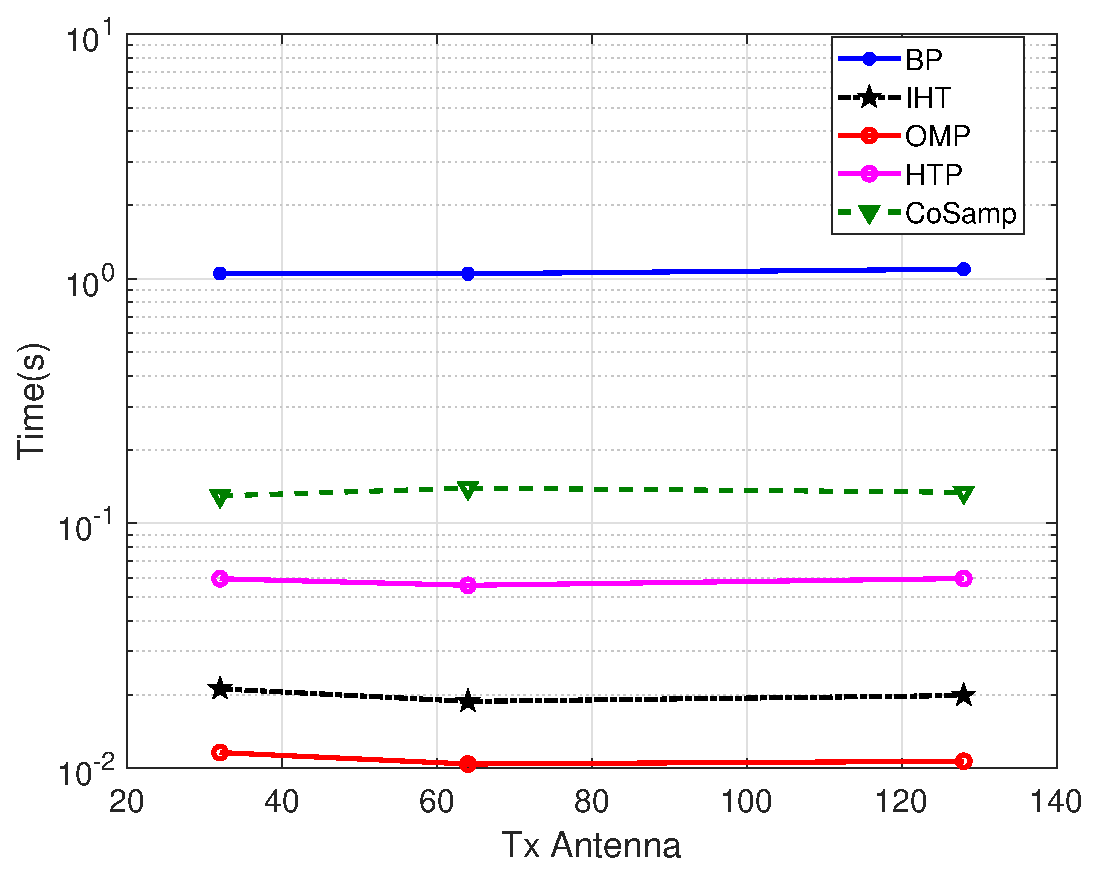
\includegraphics[width=100mm,height=75mm]{figures/figchap4/antennavstime_semilog.eps}
	\caption{Simulation time in seconds for CS techniques with \textcolor{black}{dictionary}}
	\label{FigComplex}      
\end{figure}



%\begin{figure}
%	\centering
%	\includegraphics[width=0.9\linewidth]{antennavstime_bp.eps}
%	\caption{Simulation time in seconds: BP and greedy algorithms}	
%	\label{FigComplex1}
%\end{figure}
%
%\begin{figure}
%	\centering
%	\includegraphics[width=0.9\linewidth]{antennavstime.eps}
%	\caption{Simulation time in seconds: greedy algorithms}	
%	\label{FigComplex2}
%\end{figure}

Tables \ref{tabComplexity} and Fig. \ref{FigComplex} refer to the computational complexity and the required simulation time, respectively.
%Note that \ref{FigComplex1} refers to simulation time for BP and greedy algorithms, while \ref{FigComplex2} only to the greedy algorithms to better illustrate the differences among them.

Considering Fig. \ref{Fig_result2}, \ref{FigComplex} and Table \ref{tabComplexity}, the greedy orthogonal matching pursuit and normalized hard thresholding pursuit show the best performance trade off in terms of BER and computational complexity/simulation time. Note that, although OMP shows the lowest simulation time in Fig. \ref{FigComplex}, the NHTP $BER$ performance in Fig. \ref{Fig_result2} greatly outperforms the OMP one, with a $2.5$ $dB$ gain at $10^-3$ $BER$. All the simulations are performed on an intel core i5 (7th Generation) architecture.

\section{CONCLUSION}
\label{Concl}
We have proposed a CS based channel estimation \textcolor{black}{with a suitable dictionary} for downlink beamforming in massive MIMO-OFDM FDD systems. We have exploited CS techniques to reduce training overhead, that is proportional to the sparsity level of the channel. The sparse channel representation is obtained through a \textcolor{black}{proposed dictionary} able to self-adapt to the cell characteristics. 
We have analyzed several CS algorithms in order to select among them the best technique with respect to the \textcolor{black}{proposed dictionary}. Numerical results demonstrate that basic pursuit shows the best performance at the cost of a higher complexity, while greedy solutions give good results with a lower complexity and hence shorter training period. Among them, the NHTP approach is the greedy algorithm with the best performance complexity trade-off.
